\documentclass[aspectratio=169, 14pt]{beamer}
\input{preamble}

\title{Large Language Models}
\subtitle{A Physicist's Perspective}

\begin{document}

% --- Slide 1: Title ---
\begin{frame}[plain]
  \titlepage
\end{frame}

% --- Slide 2: Section divider ---
\sectiondivider{Why this talk?}

% --- Slide 3: GPT-5.2 headline ---
\begin{frame}[plain]
  \vfill
  \centering
  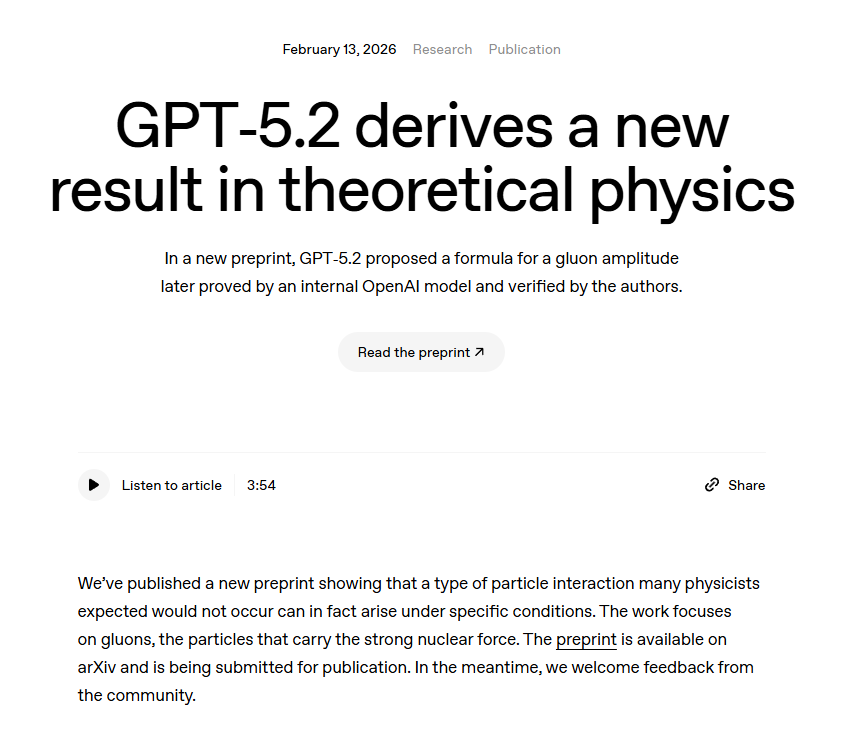
\includegraphics[width=0.85\textwidth]{assets/gpt52pr.PNG}

  \vskip1em
  {\small\color{tjo@black!60}%
    arXiv:2602.12176 \quad---\quad
    IAS, Harvard, Cambridge, Vanderbilt, OpenAI \quad---\quad
    February 2026}
  \vfill
\end{frame}

% --- Slide 4: Timeline ---
\begin{frame}{Three moments}
  \vfill
  \centering
  \begin{tikzpicture}[
    event/.style={
      tjo box,
      minimum width=3.2cm,
      minimum height=1.8cm,
      font=\normalsize,
      align=center,
    },
  ]
    % Timeline axis
    \draw[tjo@black!20, line width=2pt] (-5.5,0) -- (5.5,0);

    % Event 1: ChatGPT
    \node[event, fill=tjo@lightgrey] (gpt) at (-4,0) {%
      {\bfseries\color{tjo@darkteal} Nov 2022}\\[3pt]
      ChatGPT\\launches
    };

    % Event 2: Claude Code
    \node[event, fill=tjo@lightgrey] (cc) at (0,0) {%
      {\bfseries\color{tjo@darkteal} Q1 2025}\\[3pt]
      Claude Code,\\Cursor, Copilot
    };

    % Event 3: Models get good
    \node[event, fill=tjo@lightgrey] (good) at (4,0) {%
      {\bfseries\color{tjo@darkteal} Q4 2025}\\[3pt]
      Opus 4.5, GPT-5.2\\cross a threshold
    };
  \end{tikzpicture}
  \vfill
\end{frame}

% --- Slide 5: Audience poll ---
\begin{frame}{Quick survey: experience}
  \vfill
  \centering
  {\fontsize{20}{26}\selectfont
    \begin{tabular}{l}
      \color{tjo@cyan}$\bullet$\quad used ChatGPT, Claude, or Gemini \\[0.8em]
      \color{tjo@cyan}$\bullet$\quad used an LLM in your IDE to write code \\[0.8em]
      \color{tjo@cyan}$\bullet$\quad used a coding agent \\
    \end{tabular}
  }
  \vfill
\end{frame}

% --- Slide 6: Personal confession ---
\statementslide{If you experimented with chat in Q1 2025,\\[0.5em]
  you probably dismissed LLMs\\[0.8em]
  {\fontsize{20}{26}\selectfont\mdseries I did}}

% --- Slide 7: Skeptic ---
\statementslide{I was a skeptic\\[0.8em]
  {\fontsize{20}{26}\selectfont\mdseries
    I am still annoyed at the models of Q1 2025}}

% --- Slide 8: The problem (quote) ---
\statementslide{\textit{``LLMs are \textbf{incredibly capable}}\\[0.5em]
  \textit{but \textbf{maximally untrustworthy}''}}

% --- Slide 9: Elaboration ---
\begin{frame}{The evidence}
  \vfill
  \centering
  Seductively correct equations that are nonsense

  \vskip1.5em
  Push back on a valid proof and the LLM finds a ``bug'' that isn't there

  \vskip1.5em
  They lie, cheat, steal, and flatter

  \vskip2em
  {\color{tjo@darkteal}\bfseries All terrible qualities for reproducible science}
  \vfill
\end{frame}

% --- Slide 10: Mental model ---
\statementslide{A good mental model of an LLM:\\[0.8em]
  a slightly deranged,\\[0.3em]
  hypermotivated MSc student}

% --- Slide 11: The gap ---
\begin{frame}[plain,c]
  \centering
  {\fontsize{22}{30}\selectfont\color{tjo@darkteal}
    The gap between\\[0.6em]
    {\bfseries ``I tried ChatGPT and it hallucinated''}\\[0.6em]
    and\\[0.6em]
    {\bfseries ``this is a powerful force multiplier''}\\[0.8em]
  }
  {\fontsize{20}{26}\selectfont\color{tjo@darkteal}
    is not closed by better models\\[0.5em]
    It is closed by \textbf{technique} and \textbf{domain expertise}
  }
\end{frame}

% --- Slide 12: Three requirements ---
\begin{frame}{What it takes}
  \vfill
  \centering
  {\fontsize{20}{28}\selectfont
    \begin{tabular}{r@{\hspace{0.8em}}l}
      \color{tjo@darkteal}\bfseries 1 &
        Deliberate practice --- a different workflow \\[1em]
      \color{tjo@darkteal}\bfseries 2 &
        A subscription --- free chat is not enough \\[1em]
      \color{tjo@darkteal}\bfseries 3 &
        A coding agent --- Claude Code, Cline, \ldots \\
    \end{tabular}
  }
  \vfill
\end{frame}

% --- Slide 13: Project showcase ---
\begin{frame}{With the correct workflow}
  \vfill
  \centering
  \renewcommand{\arraystretch}{1.4}
  {\fontsize{14}{19}\selectfont
  \begin{tabular}{l@{\hspace{1.2em}}l@{\hspace{1.2em}}l}
    \textbf{\color{tjo@darkteal}vibefeld}
      & Go, 112k lines
      & adversarial proof verification \\
    \textbf{\color{tjo@darkteal}Lyr.jl}
      & Julia
      & volume renderer, GR ray tracing \\
    \textbf{\color{tjo@darkteal}af-tests}
      & Lean\,4, 0 sorries
      & formal proofs in operator algebras \\
    \textbf{\color{tjo@darkteal}convexfeld}
      & C, 37k lines
      & LP solver from scratch \\
    \textbf{\color{tjo@darkteal}Nano MIPS}
      & Verilog
      & pipelined CPU on \$10 FPGA \\
  \end{tabular}
  }

  \vskip1.5em
  {\color{tjo@darkteal}\bfseries
    All with basic tooling --- no extra subscriptions}
  \vfill
\end{frame}

% --- Slide 14: Formalization ---
\statementslide{Auto formalization is real\\[0.8em]
  Writing new science is now possible}

% --- Slide 15: Accelerating research ---
\statementslide{Accelerating research is possible\\[0.8em]
  {\fontsize{20}{26}\selectfont\mdseries
    With correct tooling and expert guidance\\[0.3em]
    The human provides the ground truth}}

% --- Slide 16: Transition ---
\statementslide{LLMs can be understood\\[0.8em]
  {\fontsize{20}{26}\selectfont\mdseries
    Let me rebuild the stack from first principles}}

\end{document}
